\clearpage
\section*{Appendix}

{
\renewcommand{\arraystretch}{1.13}
\begin{table*}[!b]
    \centering
    \vspace{-0.1in}
    \caption{Comprehensive performance comparison of \Ours and various baseline models with best values in bold and second-best underlined. MAE $\downarrow$ is specifically used as the evaluation metric. DeepSeek-R1 denotes zero-shot results using our reasoning template. Overall, \Ours achieves competitive or best performance on most datasets.}
    \label{tab:main_results_mae}
    \vspace{-0.1in}
    \resizebox{0.98\textwidth}{!}{
    \large
    \begin{tabular}{ll|ccccccccc}
        \toprule
         & \textbf{Methods}    & \textbf{ETTh1}  & \textbf{ETTh2}   & \textbf{ETTm1}   & \textbf{ETTm2}  & \textbf{Exchange} & \textbf{AQWan} & \textbf{AQShunyi} & \textbf{Wind} & \textbf{NASDAQ} \\
        \hline
        \multirow{11}{*}{Traditional} & AutoFormer & 1.5945 & 2.3246 & 2.0989 & 1.7696 & 0.0230 & 48.4358 & 51.4833 & 19.6086 & 0.0229 \\
        & PatchTST & 1.6376 & 2.0076 & 1.9446 & \underline{1.3973} & 0.0200 & \underline{39.5089} & 42.5427 & 20.4654 & \textbf{0.0213}\\
        & DLinear & 1.5116 & 2.0855 & 1.7815 & 1.9136 & 0.0256 & 51.7896 & 50.0134 & 18.6036 & 0.0217 \\
        & iTransformer & 1.5126 & 1.9295 & 1.6609 & 1.4598 & 0.0204 & 40.3070 & 42.5116 & 18.1864 & 0.0237 \\
        & TimeXer & 1.5596 & 2.0895 & 1.7785 & 1.4419 & 0.0195 & 41.8280 & 41.4929 & 18.4876 & 0.0233 \\
        & TimeMixer & \underline{1.4018} & 2.0456 & \underline{1.7103} & 1.3987 & \underline{0.0182} & 40.6789 & \textbf{40.3452} & 18.8801 & 0.0219 \\
        & WPMixer & 1.4321 & 2.0013 & 1.7502 & 1.4205 & 0.0188 & 41.2347 & \underline{40.9811} & \underline{18.1034} & 0.0225 \\
        % & TimesFM & 1.4456 & 1.9654 & 1.7345 & 1.4123 & \underline{0.0175} & 39.8765 & 41.5678 & 18.3456 & \underline{0.0215} \\
        & Moment & 1.4789 & 1.9912 & 1.7654 & 1.4456 & 0.0188 & 40.5432 & 42.1234 & 18.6789 & 0.0221 \\
        & TimesFM-2.5 & 1.4922 & 1.7195 & 2.7197 & 1.7070 & 0.0193 & 40.0290 & 43.6785 & 18.3456 & \underline{0.0215} \\
        & Chronos-2 & 1.5108 & 2.0533 & 2.5785 & 1.6766 & 0.0196 & 40.3737 & 42.3991 & 20.1270 & 0.0268 \\
        \hline
        \multirow{4}{*}{LLM-based} & CrossTimeNet & 1.5492 & 2.1731 & 1.9863 & 1.5281 & 0.0217 & 43.6267 & 46.0941 & 20.6205 & 0.0252 \\        
        & GPT4TS & 1.4299 & \underline{1.9134} & 1.9635 & 1.4943 & 0.0202 & 40.2815 & 42.3969 & 18.4919 & 0.0256 \\
        & TimeLLM & 1.4286 & 1.9143 & 1.9626 & 1.4926 & 0.0201 & 40.2746 & 42.3926 & 18.4890 & 0.0255 \\
        & DeepSeek-R1 & 1.4316 & 2.0165 & 1.8876 & 1.6289 & 0.0209 & 64.9627 & 57.6412 & 30.6469 & 0.0231 \\
        \hline
        \cellcolor{lightgray!30}Ours & \cellcolor{lightgray!30}Time-R1 & \cellcolor{lightgray!30}\textbf{1.2325} & \cellcolor{lightgray!30}\textbf{1.7192} & \cellcolor{lightgray!30}\textbf{1.6510} & \cellcolor{lightgray!30}\textbf{1.3771} & \cellcolor{lightgray!30}\textbf{0.0161} & \cellcolor{lightgray!30}\textbf{39.1846} & \cellcolor{lightgray!30}46.5032 & \cellcolor{lightgray!30}\textbf{15.1095} & \cellcolor{lightgray!30}0.0217 \\
        \bottomrule
    \end{tabular}
    }
    \vspace{-0.1in}
\end{table*}
}


\begin{figure*}[!b]
    \centering
    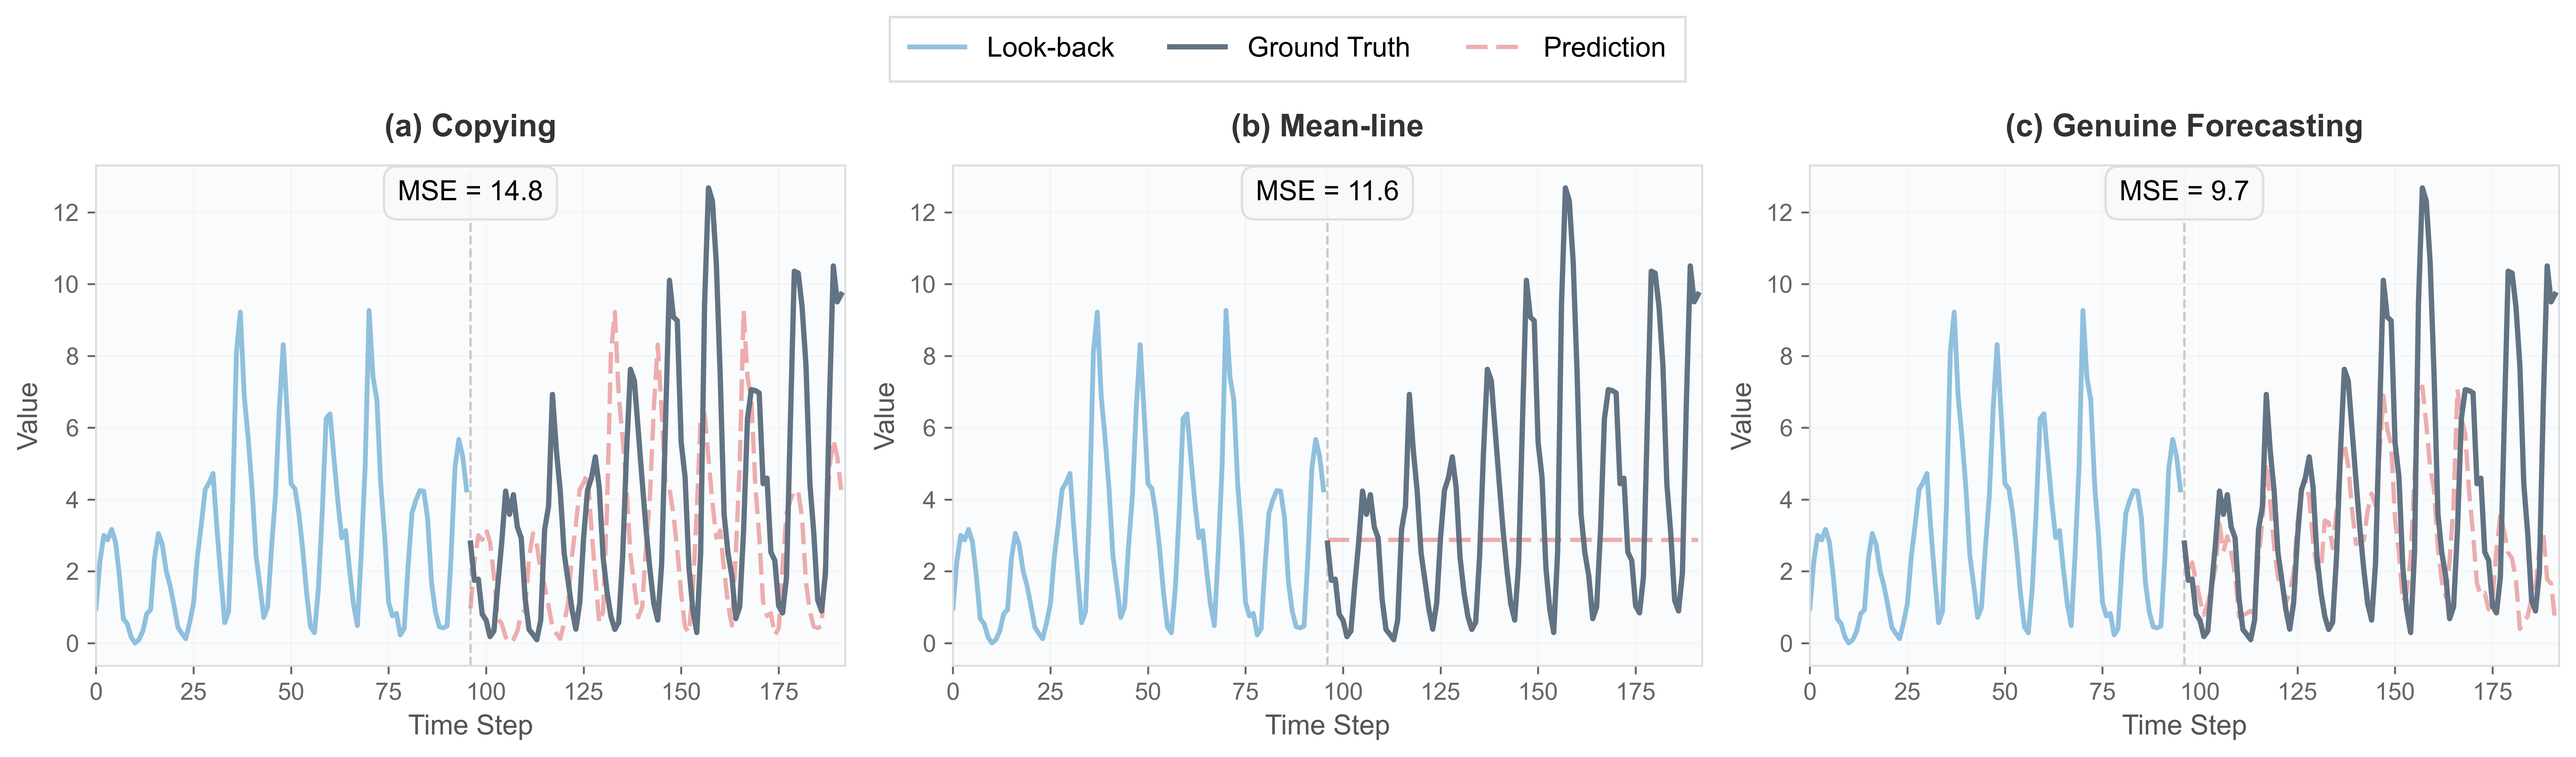
\includegraphics[width=\textwidth]{images/forecasting_comparison.png}
    \vspace{-0.3in}
    \caption{Three representative rollout modes for 96$\rightarrow$96 forecasting: 
    (a) copying the look-back window, 
    (b) mean-line output, and 
    (c) genuine forecasting. 
    Although these trajectories are qualitatively different, their MSE values can still be close enough to weaken the learning signal, especially in non-binary forecasting tasks.}

    \label{fig:forecasting_comparison}
\end{figure*}


\section{GRPO vs. GRIP: Binary-Reward Reasoning vs. Non-Binary Time-Series Forecasting} \label{section:po.vs.ip}
GRPO is well suited to reasoning tasks with \emph{verified} outcomes, such as mathematical problem solving, where rewards are nearly binary and group-relative advantages provide sharp learning signals by consistently reinforcing correct trajectories. Time-series forecasting, however, is inherently non-binary and graded under metrics such as MSE or MAE, where predictions often vary continuously in quality rather than being clearly correct or incorrect. In this setting, the reward differences among sampled completions may not reliably distinguish genuinely predictive trajectories from merely less-bad ones. More critically, when an entire sampled group consists of mediocre forecasts, the group-relative normalization in GRPO can still assign positive advantages to the relatively better samples, thereby producing misleading gradient signals that reinforce suboptimal behaviors. This may encourage ``safe'' but uninformative patterns, such as copying the look-back window or producing a flat mean-line forecast, especially when high-quality predictive trajectories are sparse. To better match this continuous reward landscape, GRIP introduces non-uniform sampling and adaptive weighting: it first explores a larger candidate pool of $k\!\cdot\!G$ trajectories, then selects $G$ trajectories through reward-weighted or diversity-preserving sampling, and finally amplifies the gradient contribution of high-reward completions rather than treating all samples equally. As illustrated in Figure \ref{fig:forecasting_comparison}, this design increases the probability of selecting and reinforcing genuine forecasting trajectories that capture trend, seasonality, and local variations.



\section{Main Results}
We present the main results using the MAE evaluation metric here in Table \ref{tab:main_results_mae}. Compared to both traditional methods and LLM-based approaches, \Ours achieves competitive improvements.


% \input{images/forecasting_comparison}
% \input{table/8_main_results_mae}



% \section{Preliminaries and Analysis of RL in LLMs}

% \subsection{Reinforcement Learning in LLMs}
% To leverage Reinforcement Learning (RL) for effectively optimizing Large Language Models (LLMs) in various Natural Language Processing (NLP) tasks, the initial and crucial step is to formulate the LLM's generation process as a Markov Decision Process (MDP)~\cite{cao2024survey, ouyang2022training}. This involves clearly defining the standard fundamental components of an RL framework: the agent, the environment, states, actions, and rewards. In this context, the LLM itself can be viewed as the agent, interacting with an environment that encompasses the specific task it is trying to solve (e.g., text generation, question answering). The agent's goal is to learn an optimal policy that maximizes a cumulative reward signal, which accurately reflects how well it performs the given task.


% \begin{figure}[h]
%     \centering
%     \includegraphics[width=\linewidth]{images/appendix_1.pdf}
%     \caption{Modeling large language models with reinforcement learning.}
%     \label{fig:rl_in_llm}
% \end{figure}

% As shown in Figure~\ref{fig:rl_in_llm}, within this MDP framework, the operationalization of RL concepts is specifically tailored to the sequential token-by-token generation characteristic of LLMs. At any discrete time step $t$, the system's current condition is captured by the state $s_t$. This state typically comprises the initial prompt concatenated with the sequence of tokens generated up to that point; thus, the initial state $s_0$ consists solely of the prompt. From a state $s_t$, the LLM executes an action $a_t$, which manifests as the selection and generation of the subsequent token from its predefined vocabulary $V$. The set of all possible tokens constitutes the action space, whose cardinality is denoted as $|V|$. The selection of a particular action $a_t$ is governed by the agent's policy $\pi(a_t|s_t)$, representing a probability distribution over the vocabulary conditional on the current state $s_t$. Following the execution of action $a_t$, the system undergoes a state transition to $s_{t+1}$. In the context of LLM generation, this transition is deterministic, defined by the concatenation $s_{t+1} = [s_t, a_t]$. Crucially for the learning process, a reward signal $r_t$ is provided, and a corresponding value function $V_t$ can be estimated. These elements are contingent upon the specific NLP objective and serve to quantify the desirability of the generated outputs or intermediate actions, thereby guiding the optimization of the LLM's policy.




% \subsection{Reinforcement Learning with Verified Reward}

% \paragraph{Group Relative Policy Optimization.}

% The GRPO method~\cite{shao2024deepseekmath} diverges from typical approaches by not requiring a critic model, which often has a comparable size to the policy model. Instead, GRPO calculates the baseline using scores obtained from a group of generated outputs.

% Specifically, for every question $q$ sampled from the dataset distribution $P(Q)$, GRPO first employs the existing policy model $\pi_{\theta_{\text{old}}}$ to produce $G$ completions, denoted as $\{o_1, o_2, \cdots, o_G\}$. Subsequently, the policy model $\pi_{\theta}$ is optimized by maximizing a defined objective:

% \begin{align}
%     \mathcal{J}_{GRPO}(\theta) = 
%     \mathbb{E}_{q \sim P(Q), \{o_i\}_{i=1}^G \sim \pi_{\theta_{old}}(o|q)}
%     \Bigg\{  
%     \frac{1}{G} \sum_{i=1}^G \frac{1}{|o_i|} \sum_{t=1}^{|o_i|} 
%     \Big\{ \min \Big[
%     \frac{\pi_\theta(o_{i,t} | q, o_{i,<t})}{\pi_{\theta_{old}}(o_{i,t} | q, o_{i,<t})} A_{i},  \notag \\
%     \text{clip} \big( \frac{\pi_\theta(o_{i,t} | q, o_{i,<t})}{\pi_{\theta_{old}}(o_{i,t} | q, o_{i,<t})}, 1 - \epsilon, 1 + \epsilon \big) A_{i} \Big] 
%     - \beta \mathbb{D}_{KL}\left[\pi_{\theta} || \pi_{ref}\right] \Big\} \Bigg\},
%     \label{eq:GRPO-obj}
% \end{align}
% \begin{equation}
%     \mathbb{D}_{KL}\left[\pi_{\theta} || \pi_{ref}\right] = 
%     \frac{\pi_{ref}(o_{i,t}|q,o_{i,<t})}{\pi_{\theta}(o_{i,t}|q,o_{i,<t})}
%     - \log\frac{\pi_{ref}(o_{i,t}|q,o_{i,<t})}{\pi_{\theta}(o_{i,t}|q,o_{i,<t})} - 1,
% \end{equation}



% In this formulation, \(\epsilon\) and \(\beta\) function as hyperparameters. The reference model is denoted by $\pi_{\theta_{\text{ref}}}$, typically representing the model's initial state before reinforcement learning is applied. Furthermore, \(A_i\) signifies the advantage, calculated from a set of rewards \(\{r_1, r_2, \dots, r_G\}\) that correspond to the various completions within each group:

% \begin{equation}
% \label{eq:advantage}
%     A_i = \frac{r_i - \mathrm{mean}(\{r_1, r_2, \dots, r_G\})}
%     {\mathrm{std}(\{r_1, r_2, \dots, r_G\})}.
% \end{equation}

% \paragraph{Rule-based Reward Function.}
% % 这里模仿 CPPO 简单介绍 reward
% Rather than relying on an auxiliary trained reward model, GRPO employs a rule-based system for reward computation. This system calculates the total reward \(r_i\) for a given output \(o_i\) by aggregating two distinct components, as formalized in Equation~\ref{eq:reward}:
% %
% \begin{equation}
% \label{eq:reward}
% 2    r_i = R_{\text{format}}(o_i) + R_{\text{accuracy}}(o_i),
% \end{equation}

% Here, the first component, the format reward \( R_{\text{format}}(o_i) \), serves to ensure that the output adheres to the required structural specifications. The second component, the accuracy reward \( R_{\text{accuracy}}(o_i) \), is designed to assign substantially higher values to responses that are correct and precise.

% \subsection{Analysis of GRPO}
% \paragraph{Analysing Training Cost and Performance Trade-off.}

% Equation \ref{eq:GRPO-obj} reveals a linear relationship between GRPO's training overhead and the number of sampled completions. This is primarily due to the necessity of computing probability distributions over all completions for the policy, reference, and old policy models. Taking the DeepSeek-Math experiment as an example, sampling 16 completions per question requires 48 forward passes (16 × 3), leading to a sharp increase in computational cost. Experimental results (Figure \ref{fig:mse}) show that increasing the number of completions can improve model MSE and MAE on the ETTh1 dataset, with diminishing returns in performance gains. More critically, reducing the number of completions to lower computational load significantly degrades the reasoning capability of the Qwen2.5-7B-Instruct model, highlighting the limitations of conventional approaches.

% \paragraph{Analyzing Optimization Opportunities from Contribution Heterogeneity.}

% Recent work \cite{lin2025cppo} reveals substantial heterogeneity in the contribution of individual completions to the overall training effectiveness. A small subset of high-value samples can typically provide optimization signals up to tens of times stronger than ordinary ones. This non-uniform distribution opens new avenues for improving training efficiency: by dynamically identifying and prioritizing high-contribution samples, it becomes possible to significantly reduce computational overhead to as low as one-third or even one-fifth of the original level while maintaining model performance (see Section \ref{sec:GRIP} for detailed optimization strategies). These findings not only explain the efficiency bottlenecks in existing methods but also lay a robust theoretical foundation for the design of adaptive sampling strategies in promising future work.



% \clearpage
% \paragraph{Analysising Completion Contribution.}
% To accurately evaluate the contribution of each individual completion to the training of the underlying policy model, we analyze the specific derivative structure of the objective function presented in Eq.\,(\ref{eq:GRPO-obj}) with respect to the trainable model parameters $\theta$ as:

% \begin{equation}
% \begin{aligned}
%  \nabla_{\theta} J_{GRPO}(\theta)=&\,\mathbb{E}_{\left[q \sim P(Q), \{o_{i}\}_{i=1}^{G} \sim \pi_{\theta_{old}}(O|q)\right]} \Bigg\{ \frac{1}{G} \sum_{i=1}^{G} \frac{1}{\left|o_{i}\right|} \sum_{t=1}^{\left|o_{i}\right|} \Bigg[ \nabla_{\theta}\left(\frac{\pi_{\theta}\left(o_{i, t} | q, o_{i,<t}\right)}{\pi_{\theta_{old}}\left(o_{i, t} | q, o_{i,<t}\right)} A_i\right) \\
% &\quad\quad\quad\quad - \beta\left(\nabla_{\theta} \frac{\pi_{r e f}\left(o_{i, t} | q, o_{i,<t}\right)}{\pi_{\theta}\left(o_{i, t} | q, o_{i,<t}\right)}-\nabla_{\theta} \log \frac{\pi_{r e f}\left(o_{i, t} | q, o_{i,<t}\right)}{\pi_{\theta}\left(o_{i, t} | q, o_{i,<t}\right)}\right) \Bigg]\Bigg\} \\
% %
% =&\mathbb{E}_{\left[q \sim P(Q), \{o_{i}\}_{i=1}^{G} \sim \pi_{\theta_{old}}(O|q)\right]} \Bigg\{ \frac{1}{G} \sum_{i=1}^{G} \frac{1}{\left|o_{i}\right|} \sum_{t=1}^{\left|o_{i}\right|} \Bigg[ \frac{\nabla_{\theta} \pi_{\theta}\left(o_{i, t} | q, o_{i,<t}\right)}{\pi_{\theta_{old}\left(o_{i, t} | q, o_{i,<t}\right)}}A_i \\
% &+ \beta\left(\frac{\pi_{r e f}\left(o_{i, t} | q, o_{i,<t}\right)\nabla_{\theta} \pi_{\theta}\left(o_{i, t} | q, o_{i,<t}\right)}{\pi_{\theta}^{2}\left(o_{i, t} | q, o_{i,<t}\right)} - \frac{\nabla_{\theta} \pi_{\theta}\left(o_{i, t} | q, o_{i,<t}\right)}{\pi_{\theta}\left(o_{i, t} | q, o_{i,<t}\right)}\right) \Bigg] \Bigg\} \\
% %
% =&\mathbb{E}_{\left[q \sim P(Q), \{o_{i}\}_{i=1}^{G} \sim \pi_{\theta_{old}}(O|q)\right]} \Bigg\{  \frac{1}{G} \sum_{i=1}^{G} \frac{1}{\left|o_{i}\right|} \sum_{t=1}^{\left|o_{i}\right|} \Bigg[ \frac{\pi_{\theta}\left(o_{i, t} | q, o_{i,<t}\right)}{\pi_{\theta_{old}}\left(o_{i, t} | q, o_{i,<t}\right)} A_i  \\ 
% &\quad\quad\quad\quad\quad\quad\quad + \beta\left(\frac{\pi_{r e f}\left(o_{i, t} | q, o_{i,<t}\right)}{\pi_{\theta}\left(o_{i, t} | q, o_{i,<t}\right)} - 1\right)\Bigg] \frac{\nabla_{\theta} \pi_{\theta}\left(o_{i, t} | q, o_{i,<t}\right)}{\pi_{\theta}\left(o_{i, t} | q, o_{i,<t}\right)}\Bigg\} \\
% %
% =&\mathbb{E}_{\left[q \sim P(Q), \{o_{i}\}_{i=1}^{G} \sim \pi_{\theta_{old}}(O|q)\right]} \Bigg\{ \frac{1}{G} \sum_{i=1}^{G} \frac{1}{\left|o_{i}\right|} \sum_{t=1}^{\left|o_{i}\right|} \Bigg[  \underbrace{\frac{\pi_{\theta}\left(o_{i, t} | q, o_{i,<t}\right)}{\pi_{\theta_{old}}\left(o_{i, t} | q, o_{i,<t}\right)}}_{
% \textit{Probability ratio}} \underbrace{A_i }_{\textit{Advantage}}\\ 
% &\quad\quad\quad\quad\quad + \underbrace{\beta\left(\frac{\pi_{r e f}\left(o_{i, t} | q, o_{i,<t}\right)}{\pi_{\theta}\left(o_{i, t} | q, o_{i,<t}\right)}-1\right)}_{\textit{KL divergence constraint}}   \Bigg] \underbrace{\nabla_{\theta} \log \pi_{\theta}\left(o_{i, t} | q, o_{i,<t}\right)}_{
% \textit{Policy model gradient}}\Bigg\}.
% \end{aligned}
% \label{eq:GRPO-obj-derivative}
% \end{equation}
% %




% This analysis reveals four key factors influencing policy updates:  



% 1. \textbf{\textit{Advantage}}, which assesses the value of a completion in improving expected returns through the advantage function. A higher advantage indicates stronger reward alignment, making the completion more influential in guiding policy updates.

% 2. \textbf{\textit{Probability ratio}}, wich compares the likelihood of an action under the current policy $\pi_\theta$ to that under the old policy $\pi_{\theta_{\text{old}}}$. It amplifies actions favored by the new policy and suppresses those preferred by the old one, guiding the policy toward higher rewards. A higher ratio signifies greater confidence in the action, influencing the optimization process more significantly. This term is crucial for identifying high-value completions when combined with the advantage function.

% 3. \textbf{\textit{KL divergence}}, which measures the deviation of the current policy from the reference model. It enforces stability during training by penalizing excessive changes, but does not directly contribute to reasoning pattern formation.

% 4. \textbf{\textit{Policy model gradient}}, which indicates the direction of parameter updates.

% Previous research \cite{hu2025open} has shown that removing the KL divergence constraint does not significantly affect the model's reasoning performance, as the core learning signal primarily comes from the advantage term aligned with rewards. Furthermore, we can effectively decompose the core mathematical expression for policy updates into two distinct components: the \textit{probability ratio} and the \textit{advantage} term. For a specific completion to make a significant contribution to training, both components must simultaneously have substantial values. If either of them is close to zero, the overall contribution will also be naturally negligible. 
% By removing the KL divergence term and decoupling its regularization effect, we derive the simplified form of GRPO’s objective derivative as:

% \begin{equation}
% \begin{aligned}
% \nabla_{\theta} J_{GRPO}(\theta) &  \approx  \, \mathbb{E}_{\left[q \sim P(Q), \{o_{i}\}_{i=1}^{G} \sim \pi_{\theta_{old}}(O|q)\right]} \\
% &\Bigg\{ \frac{1}{G} \sum_{i=1}^{G} \frac{1}{\left|o_{i}\right|} \sum_{t=1}^{\left|o_{i}\right|} \Big[ \underbrace{\frac{\pi_{\theta}\left(o_{i, t} | q, o_{i,<t}\right)}{\pi_{\theta_{old}}\left(o_{i, t} | q, o_{i,<t}\right)} }_{\substack{\textit{Probability ratio}}}\cdot \underbrace{A_i}_{\substack{\textit{Advantage}}}  \Big] \underbrace{\nabla_{\theta} \log \pi_{\theta}\left(o_{i, t} | q, o_{i,<t}\right)}_{\substack{\textit{Policy model gradient}}} \Bigg\},
% \end{aligned}
% \label{eq:GRPO-obj-derivative-2}
% \end{equation}

% This simplified formulation focuses on the reward-driven learning signal while preserving the essential gradient dynamics required for effective policy optimization. With the help of this simplified expression, we can evaluate the advantage value of each completion before the full model computation is carried out. Specifically, if a completion exhibits a very small absolute advantage value, its contribution to the policy update is negligible. We can filter out such low-value completions at an early stage, thereby avoiding redundant forward and backward computations.

% To further improve training efficiency and learning effectiveness, we could introduce a sampling strategy based on reward values or advantage estimates. Unlike uniform sampling across all completions, we prioritize those with higher advantage values for inclusion in the training process. These samples typically contain stronger learning signals and are more valuable for policy updates. By increasing the sampling probability of these high-impact completions during batch construction—or through upsampling techniques—we not only reduce computational overhead but also significantly accelerate convergence and enhance final model performance.

% This approach ensures efficient training iterations while maintaining the quality of policy updates, achieving a favorable balance between computational cost and learning effectiveness. As a result, it enables a dual improvement in both training efficiency and model capability.

% \section{Group-based Relative Importance for Policy Optimization}
% \label{sec:GRIP}

% We introduce GRIP (Group-based Relative Importance for Policy Optimization), a general RL optimization method designed for optimizing entire trajectories generated by LLMs  as time series forecasting reasoners. Unlike GRPO, which linearly increases inference cost with the number of completions due to uniform sampling and equal weighting, GRIP adopts a non-uniform sampling strategy that selects a small subset of high-reward trajectories from a larger candidate pool, significantly reducing forward passes. Furthermore, GRIP employs adaptive weighting to amplify gradient signals from informative samples, enabling more efficient learning from high-value completions. This design not only reduces compute burden but also mitigates the diminishing returns of increased sample count, thereby enhancing both training efficiency and forecasting accuracy. The GRIP objective function, formally defined in Equation~\ref{eq:grip}, operates within a policy gradient framework and integrates a non-uniform sampling strategy with adaptive trajectory weighting.
% \begin{align}
% \mathcal{J}_{\text{GRIP}}(\theta) = 
% &\mathbb{E}_{\substack{q \sim P(Q), \\ \{o_j\}_{j=1}^{k \cdot G} \sim \pi_{\theta_{\text{old}}}(o|q), \\ \{o_i\}_{i=1}^G \sim \text{Sample}\left(\{o_j\}_{j=1}^{k \cdot G}; R(o_j)\right)}} 
% \Bigg\{ 
% \sum_{i=1}^{G} w_i^U  
% \frac{1}{|o_i|} 
% \bigg\{
% \sum_{t=1}^{|o_i|} 
% \min\bigg[ 
% \frac{\pi_\theta(o_{i,t}|q, o_{i,<t})}{\pi_{\theta_{\text{old}}}(o_{i,t}|q, o_{i,<t})} A_i,\nonumber\\
% &
% \text{clip}\Big( \frac{\pi_\theta(o_{i,t}|q, o_{i,<t})}{\pi_{\theta_{\text{old}}}(o_{i,t}|q, o_{i,<t})}, 1-\epsilon, 1+\epsilon \Big) A_i 
% \bigg]
% - \beta \mathbb{D}_{KL} [\pi_\theta || \pi_{ref}] 
% \bigg\} 
% \Bigg\}.
% \label{eq:grip}
% \end{align}  
% where $\epsilon$ and $\beta$ are hyperparameters. $\pi_{\text{ref}}$ is the reference model, typically initialized as the pre-trained model before reinforcement learning begins. The output $\{o_i\}$ is selected through a sampling process from policy $\pi_{\theta_{\text{old}}}$. The hyperparameter $k$ controls the size of the rollout space, while $G$ referred to as the group size. $\mathbb{D}_{KL}$ represents the KL divergence, which is incorporated into the loss function as a regularization term during training. And $A_i$ is the advantage computed using a group of rewards $\{r_1, r_2, \dots, r_G\}$ corresponding to the completion trajectories within each group.
% The weight $w_i^U$ denotes the adaptive weighting assigned to each trajectory. This objective balances exploration and exploitation while mitigating gradient dilution. The sampling strategy and adaptive weight will be discussed in the following section.



% \subsection{GRIP Pipeline}
% To elucidate its operational mechanics, the GRIP algorithm is implemented through a structured pipeline. The distinct stages of this process are outlined as follows:
% %

% (1) The old policy model samples $k$ groups of $G$ completions for each question, a total of $k\cdot G$.

% (2) The reward function computes the reward for each completion (Sec. \ref{sec:Reward Modeling}).

% (3) GRIP non-uniformly samples $G$ completions based on rewards to balance exploration and exploitation (Sec. \ref{sec:sampling}).

% (4) The advantage of each completion is calculated, and adaptive weighting is employed to assign greater significance to high-quality reasoning paths among these completions (Sec. \ref{sec:Adaptive Weighting}).

% (5) Subsequently, the policy model is updated, with its gradient signals effectively formed as a weighted average of the selected completions, reflecting this assigned path-dependent significance.


% GRIP differs significantly from GRPO in both its initial sampling strategy and the mechanism for weighting completion contributions during policy updates. GRPO typically generates $G$ completions directly and employs an arithmetic mean when processing their outcomes. In contrast, GRIP first explores a broader set by sampling $k \cdot G$ completions, from which $G$ are subsequently selected for the update phase. Critically, while GRPO's use of an arithmetic mean implies equal consideration for its $G$ samples, GRIP's policy update leverages an adaptive weighted average. This ensures that high-quality reasoning paths within the selected $G$ completions exert a more substantial influence on the gradient signals, thereby fostering more robust and effective learning.

% \section{GRPO vs. GRIP: Binary-Reward Reasoning vs. Non-Binary Time-Series Forecasting} \label{section:po.vs.ip}
% GRPO was originally developed and widely validated in reasoning tasks with \emph{verified} outcomes such as mathematical problem solving, where the reward is close to binary an answer is either correct or incorrect. In such settings, the group-relative advantage provides a sharp learning signal: trajectories that solve the problem receive consistently higher rewards and are repeatedly reinforced, leading to stable improvement. However, time series forecasting differs fundamentally: evaluation is inherently non-binary and graded (e.g., MSE/MAE), and many outputs can be "partially correct". This makes the reward landscape smoother and the gap between mediocre and truly correct forecasts much smaller, so the uniform sampling and equal treatment of completions can dilute gradient signals and encourage exploitation of "safe" but uninformative behaviors. In practice, the policy may collapse to trivial patterns that minimize loss without genuine forecasting, such as copying the look-back window verbatim, or outputting a flat line near the historical mean especially when high-quality predictive trajectories are sparse.

% To address this mismatch, GRIP introduces a non-uniform sampling and adaptive weighting mechanism that explicitly prioritizes rare but high-reward forecasting trajectories. Concretely, instead of drawing only $G$ completions and averaging them as in GRPO, GRIP first explores a larger candidate pool ($k\!\cdot\!G$) and then selects $G$ trajectories via reward-weighted (or diversity-preserving) sampling for policy updates; meanwhile, an adaptive weighted average amplifies the gradient contribution of high-quality completions, rather than assigning all samples equal importance. Figure \ref{fig:forecasting_comparison} illustrates three representative rollout modes observed during optimization: (i) a \emph{copying} mode that repeats the input window, (ii) a \emph{mean-line} mode that outputs an almost constant sequence, and (iii) a \emph{genuine forecasting} mode that extrapolates trend/seasonality and reacts to local changes, where GRIP increases the probability of selecting and reinforcing the third mode during training.




% \section{CoT-based Supervised Fine-tuning Data collection}
% \label{sec:SFT}
% \begin{algorithm}
% \caption{Three-stage CoT data construction for \textsc{Ours}}
% \label{alg:cot_construction}
% \begin{algorithmic}[1]
% \STATE \textbf{Input:} $\mathcal{T}$ := Set of training time series samples with historical data and ground truth labels  
% \STATE \textbf{Output:} $\mathcal{D}_{\text{SFT}}$ := Structured Chain-of-Thought dataset for SFT  
% \STATE $\mathcal{D}_{\text{SFT}} \gets \emptyset$ \hfill \textit{Initialize the output dataset}

% \FOR{$t \in \mathcal{T}$}
%     \STATE $x_{\text{hist}} \gets \text{ExtractHistorical}(t)$ 
%     \STATE \hfill \textit{Extract historical time series input}
    
%     \STATE $y_{\text{pred}}^{(1)}, \dots, y_{\text{pred}}^{(k)} \gets \text{DeepSeek-R1}(x_{\text{hist}}; \text{strict formatting})$ 
%     \STATE \hfill \textit{Generate $k$ candidate predictions}
    
%     \STATE $\text{MAPE}_i \gets \text{ComputeMAPE}(y_{\text{pred}}^{(i)}, y_{\text{true}})$ for each candidate 
%     \STATE \hfill \textit{Evaluate using MAPE}
    
%     \STATE $y^* \gets \text{SelectMinMAPE}(\{y_{\text{pred}}^{(i)}\})$ 
%     \STATE \hfill \textit{Select best prediction}
    
%     \STATE $\text{CoT}^{(1)}, \dots, \text{CoT}^{(k)} \gets \text{DeepSeek-R1}(\text{prompt}=x_{\text{hist}}, y_{\text{true}}, \text{CoT of $y^*$})$ 
%     \STATE \hfill \textit{Prompt to generate reasoning paths based on ground truth label}
    
%     \STATE $\text{CoT}^* \gets \text{SelectHighQuality}(\{\text{CoT}^{(i)}\}, y_{\text{true}})$ 
%     \STATE \hfill \textit{Select CoT aligned with ground truth label}
    
%     \STATE $\text{sample} \gets \text{Concatenate}(\text{\textless think\textgreater}, \text{CoT}^*, \text{\textless \textbackslash think\textgreater}, \text{\textless answer\textgreater},  y_{\text{true}}, \text{\textless \textbackslash answer\textgreater})$ 
%     \STATE \hfill \textit{Combine reasoning and true answer}
    
%     \STATE $\mathcal{D}_{\text{SFT}} \gets \mathcal{D}_{\text{SFT}} \cup \{\text{sample}\}$ 
%     \STATE \hfill \textit{Add to final dataset}
% \ENDFOR

% \end{algorithmic}
% \end{algorithm}

% \section{Data Statistics}
% \label{dataset}
% We presents the statistical characteristics of our datasets, shown in table \ref{tab:data_statistics}.
% % \begin{table}[th]
%     \centering
%     \large
%     \caption{Statistics information of experimental datasets.}
%     % \vspace{-0.06in}
%     \renewcommand{\arraystretch}{1.3}
%     \scalebox{0.7}{
%     \begin{tabular}{cccccccccc}
%     \hline
%         Dataset & Domain & Timestamps & Features &  Frequency \\ 
%         \hline
%         ETTh1\&ETTh2 & Electricity & 17,420 & 7 &  1 hour \\ 
%         ETTm1\&ETTm2 & Electricity & 69,680 & 7 &   15 mins \\
%         AQWan\&AQShunyi & Environment & 35,064 & 11 & 1 hour  \\ 
%         Exchange & Economy & 7,588 & 8 &  1 day  \\ 
%         Wind & Energy & 48,673 & 7 &   15 mins \\ 
%         NASDAQ & Stock & 1,244 & 5 &  1 day \\ 
%     \hline
%     \end{tabular}
%     }
%     \label{tab:data_statistics}
% \end{table}



\begin{table}[t]\centering
    \caption{Statistics information of experimental datasets.}
    \renewcommand{\arraystretch}{1.2}
    \vspace{-0.1in}
    \label{tab:data_statistics}
    \resizebox{0.48\textwidth}{!}{
    \large
    \begin{tabular}{cccccccccc}
        \toprule
        Dataset & Domain & Timestamps & Features &  Frequency \\ 
        \hline
        ETTh1\&ETTh2 & Electricity & 17,420 & 7 &  1 hour \\ 
        ETTm1\&ETTm2 & Electricity & 69,680 & 7 &   15 mins \\
        AQWan\&AQShunyi & Environment & 35,064 & 11 & 1 hour  \\ 
        Exchange & Economy & 7,588 & 8 &  1 day  \\ 
        Wind & Energy & 48,673 & 7 &   15 mins \\ 
        NASDAQ & Stock & 1,244 & 5 &  1 day \\ 
        \bottomrule
    \end{tabular}
    }
    \vspace{-0.2in}
\end{table}


% \section{Additional Result and Analysis}

% \subsection{Main Results}
% Due to page limitations, we present the main results using the MAE evaluation metric here in Table \ref{tab:main_results_mae}. Compared to both traditional methods and LLM-based approaches, \Ours achieves competitive improvements.



% \input{images/6_ts_case}
% \subsection{Visualization of Prediction Results}
% In this visualization (Figure \ref{fig:ts_case}), \Ours is compared against six baseline methods, including LLM-based approaches (GPT4TS and TimeLLM) and traditional models (PatchTST, iTransformer, Autoformer, and TimeXer). \Ours consistently demonstrates more accurate and smoother predictions, closely aligning with the ground truth. In contrast, the version of \Ours trained with only SFT performs poorly, yielding subpar forecasting results. On the other hand, \Ours with only RL achieves improved performance, outperforming the baselines to some extent.

% \subsection{Analysis about Reward Design}
% \label{more_reward}
% % \paragraph{Distance Metric in Accuracy Reward.}
% To investigate the impact of different distance metrics on the accuracy reward during the reinforcement learning phase, we conducted experiments on multiple real-world time series forecasting tasks using the Exchange, AQShunyi, and NASDAQ datasets, shown in Figure \ref{fig:distance_metrics}. Specifically, we evaluated Mean Squared Error (MSE), Mean Absolute Error (MAE), Dynamic Time Warping (DTW), and Mean Absolute Percentage Error (MAPE) as accuracy reward signals within our GRIP optimization framework. The experimental results demonstrate that MSE consistently outperformed other metrics, followed by MAE, while DTW and MAPE showed relatively limited improvements.
% MSE penalizes the squared prediction errors, making it more sensitive to outliers, thereby guiding the model to focus on overall consistency between predictions and ground truth values. This leads to enhanced stability in multi-step forecasts. In contrast, although MAE is more robust due to its linear response to errors, it suffers from less concentrated gradient updates, affecting convergence efficiency. DTW, despite its ability to handle temporal misalignment, introduces computational complexity and asymmetry issues, making it challenging to integrate effectively into end-to-end training. Additionally, MAPE can suffer from numerical instability when target values are close to zero, limiting its practical utility in training.
% In conclusion, we recommend prioritizing MSE as the primary accuracy reward metric during the reinforcement learning optimization phase to achieve superior predictive accuracy and reasoning stability. Auxiliary reward terms can be incorporated based on specific task requirements to further enhance the robustness of the model.

% \begin{figure*}[h] \centering
    
    \makebox[0.32\textwidth]{ Exchange Dataset}
    \hspace{0.01\textwidth}
    \makebox[0.32\textwidth]{ AQShunyi Dataset}
    \hspace{0.02\textwidth}
    \makebox[0.31\textwidth]{ NASDAQ Dataset}
    \\
    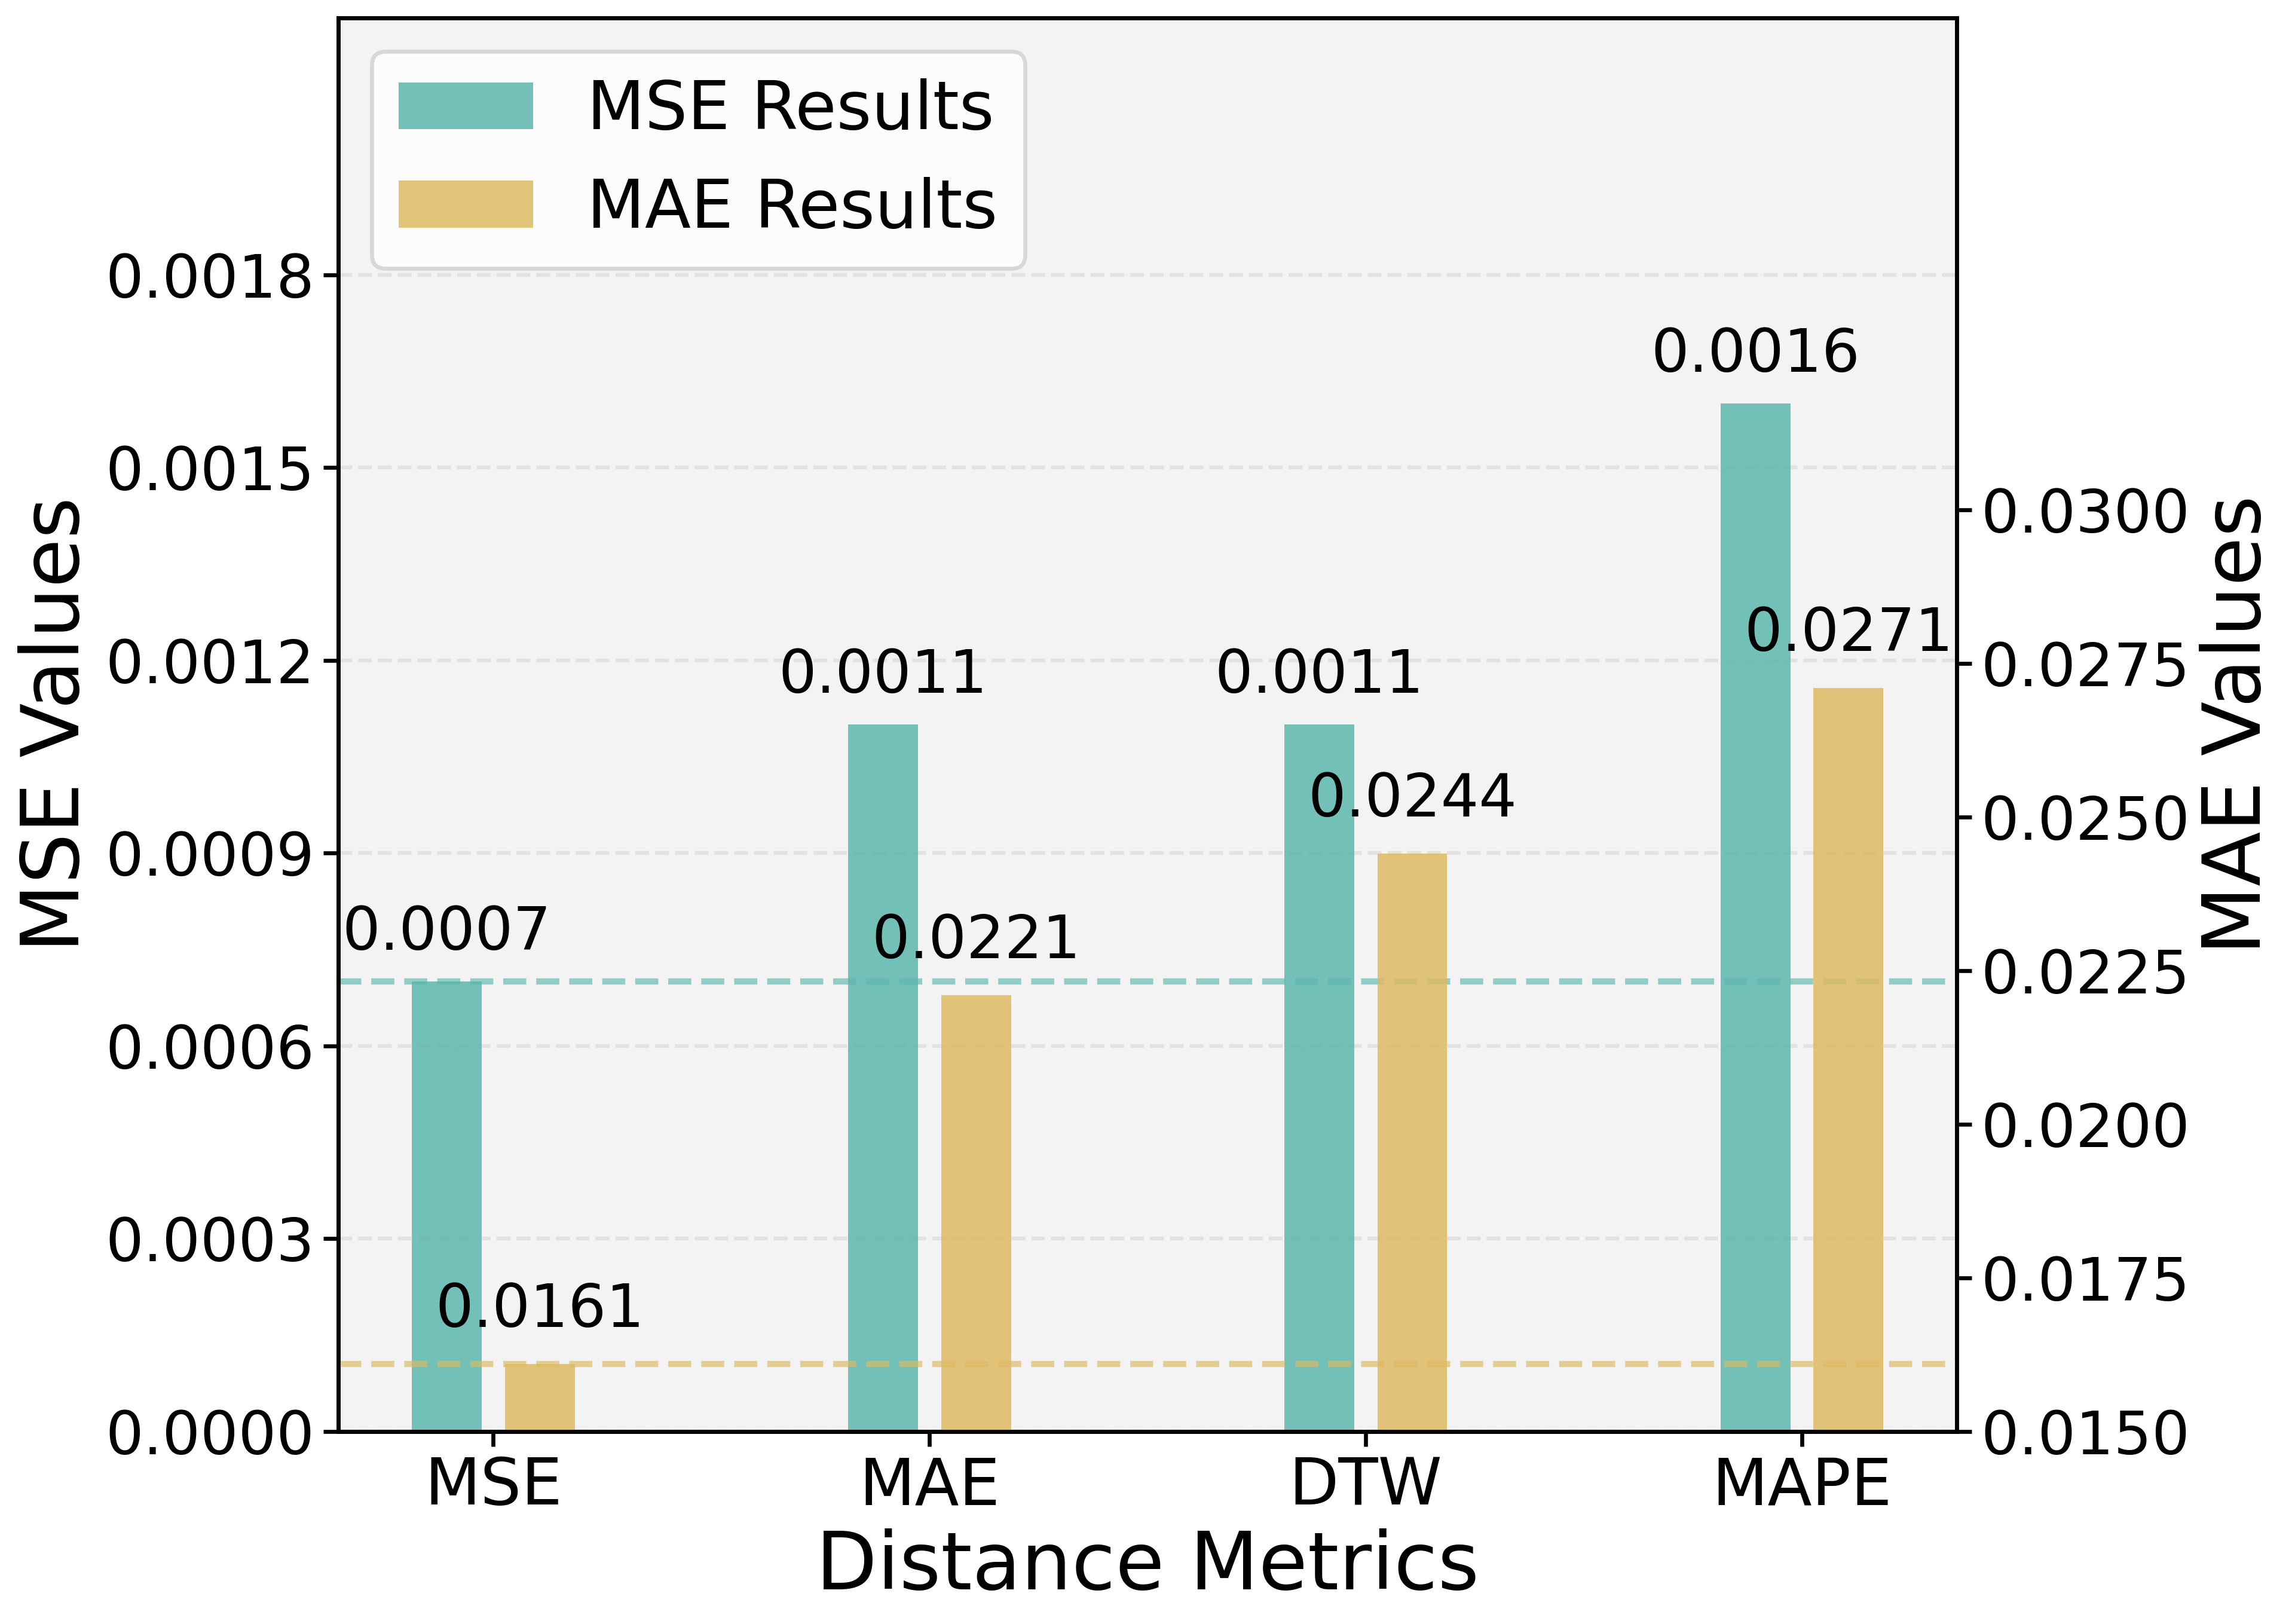
\includegraphics[width=0.32\textwidth]{images/distance/Exchange_results.png}
     \hspace{0.01\textwidth}
    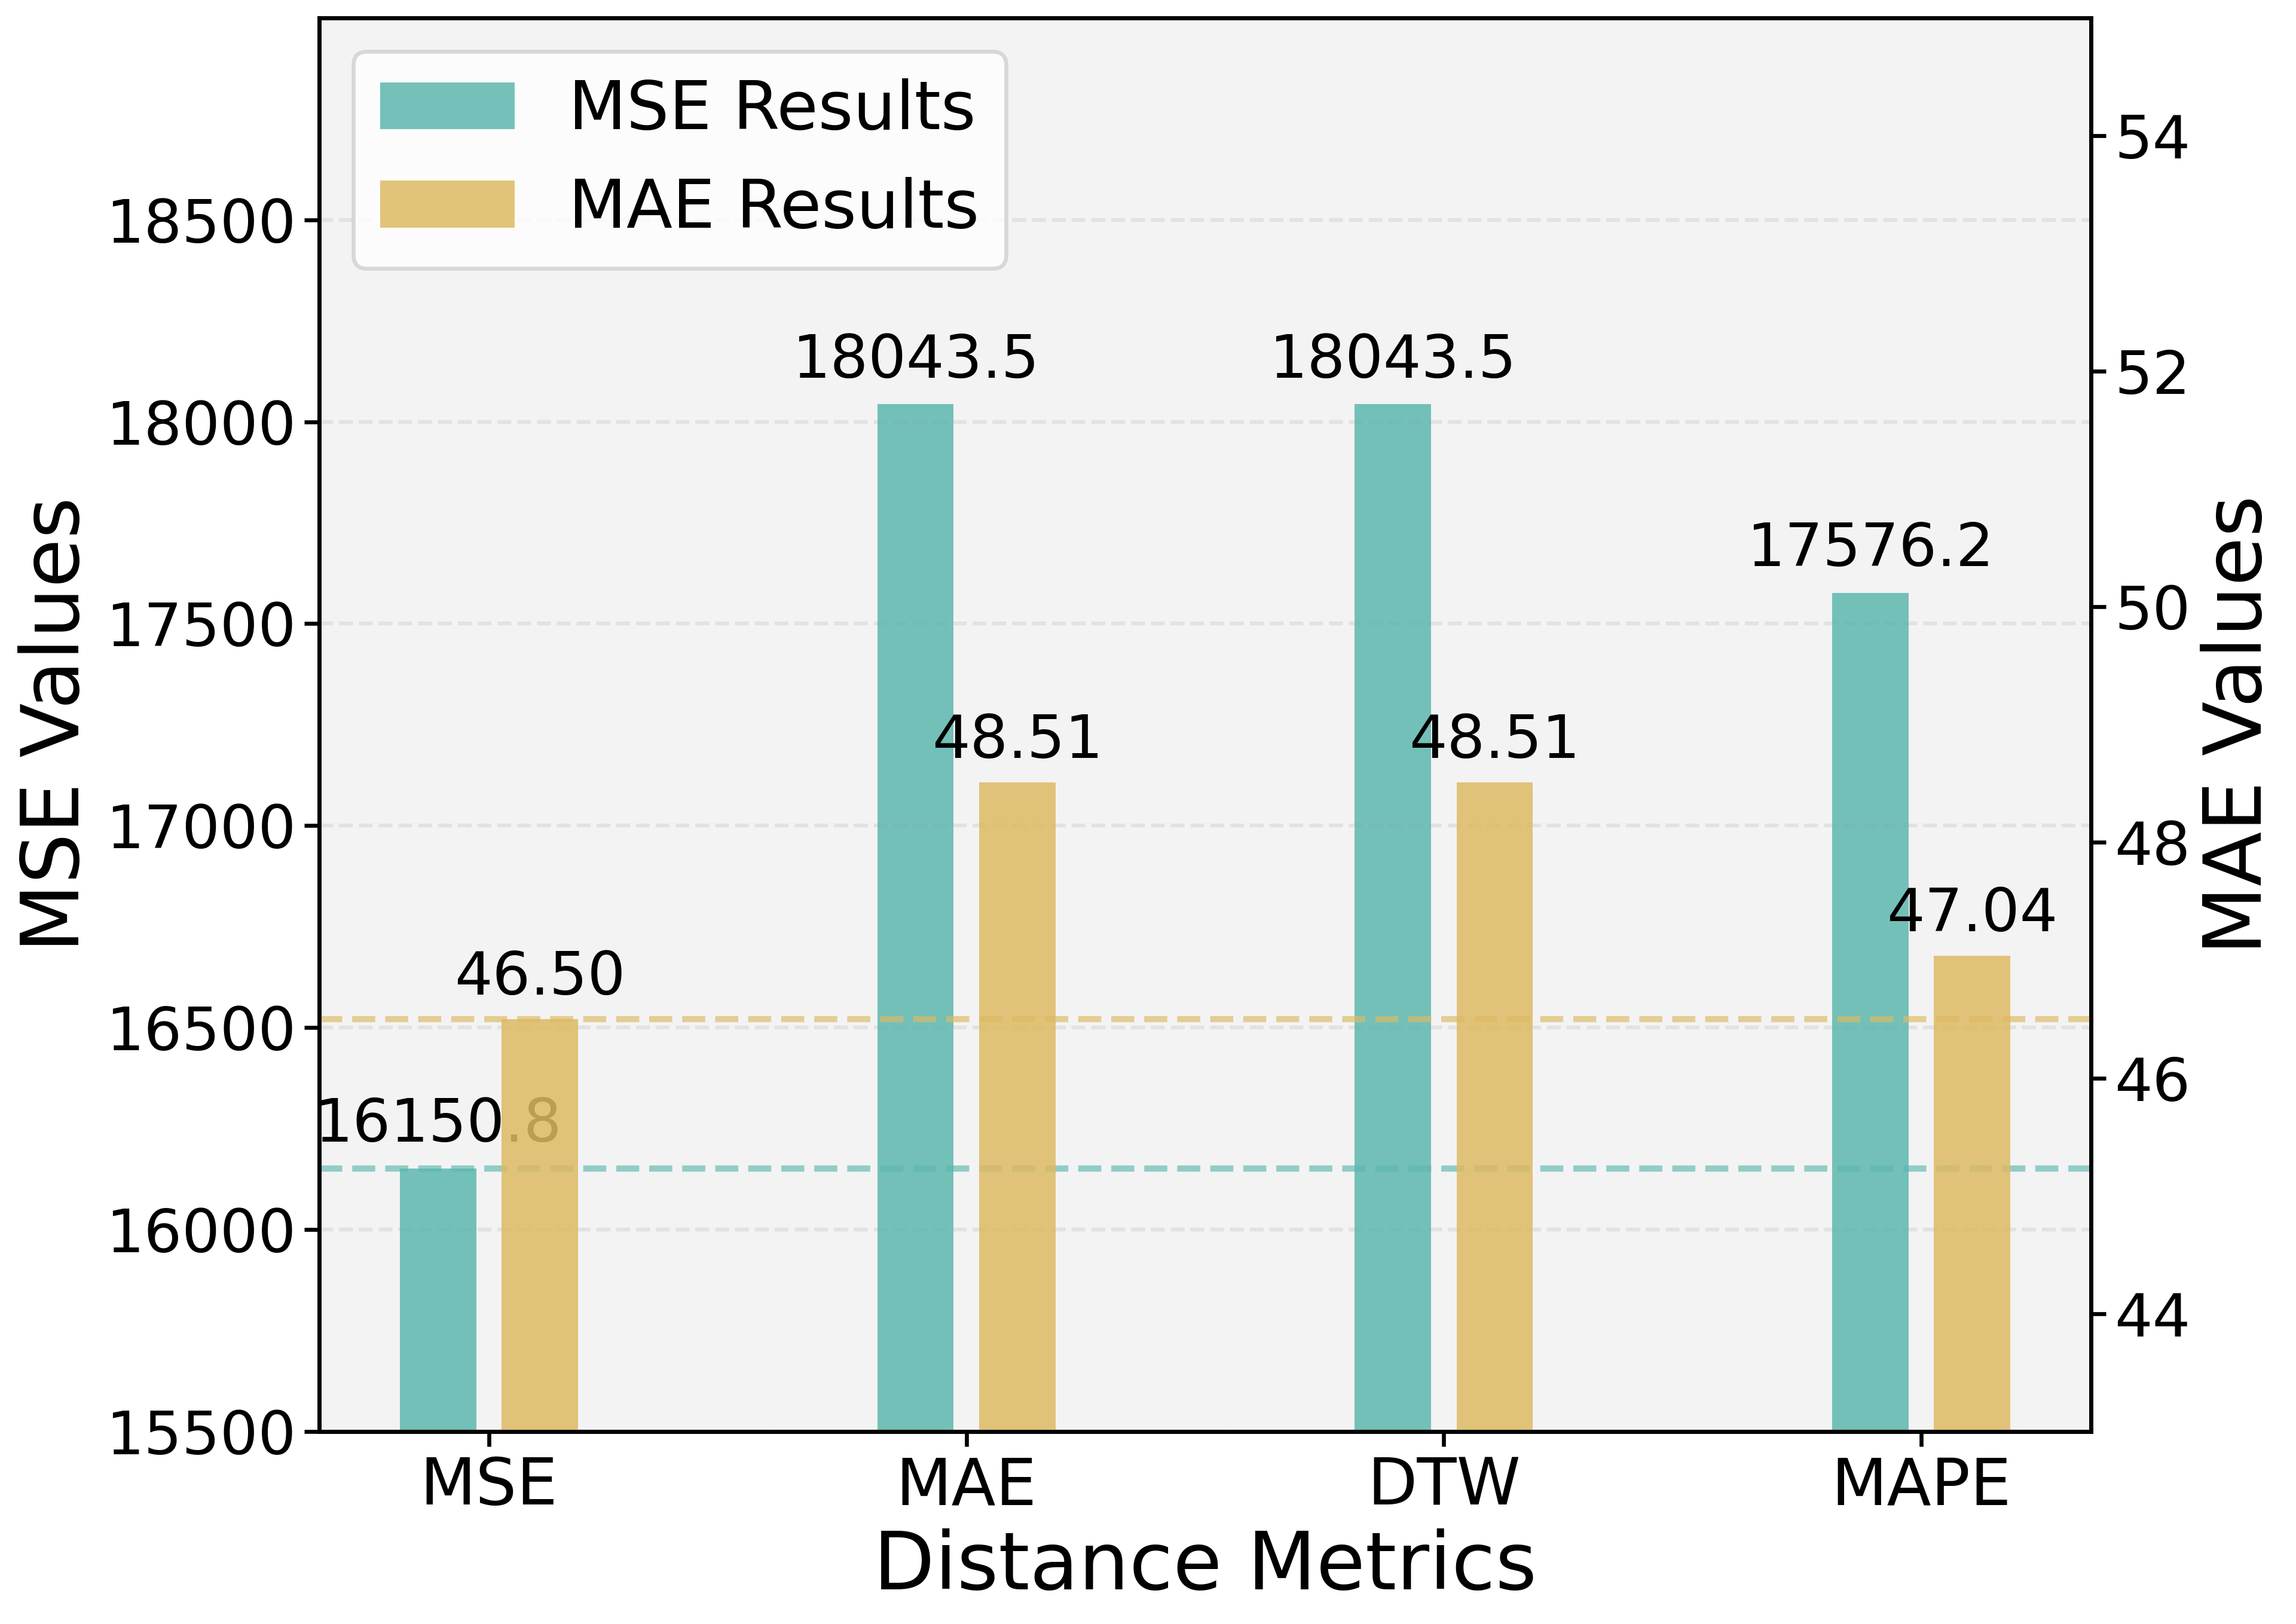
\includegraphics[width=0.32\textwidth]{images/distance/AQShunyi_results.png}
    \hspace{0.01\textwidth}
    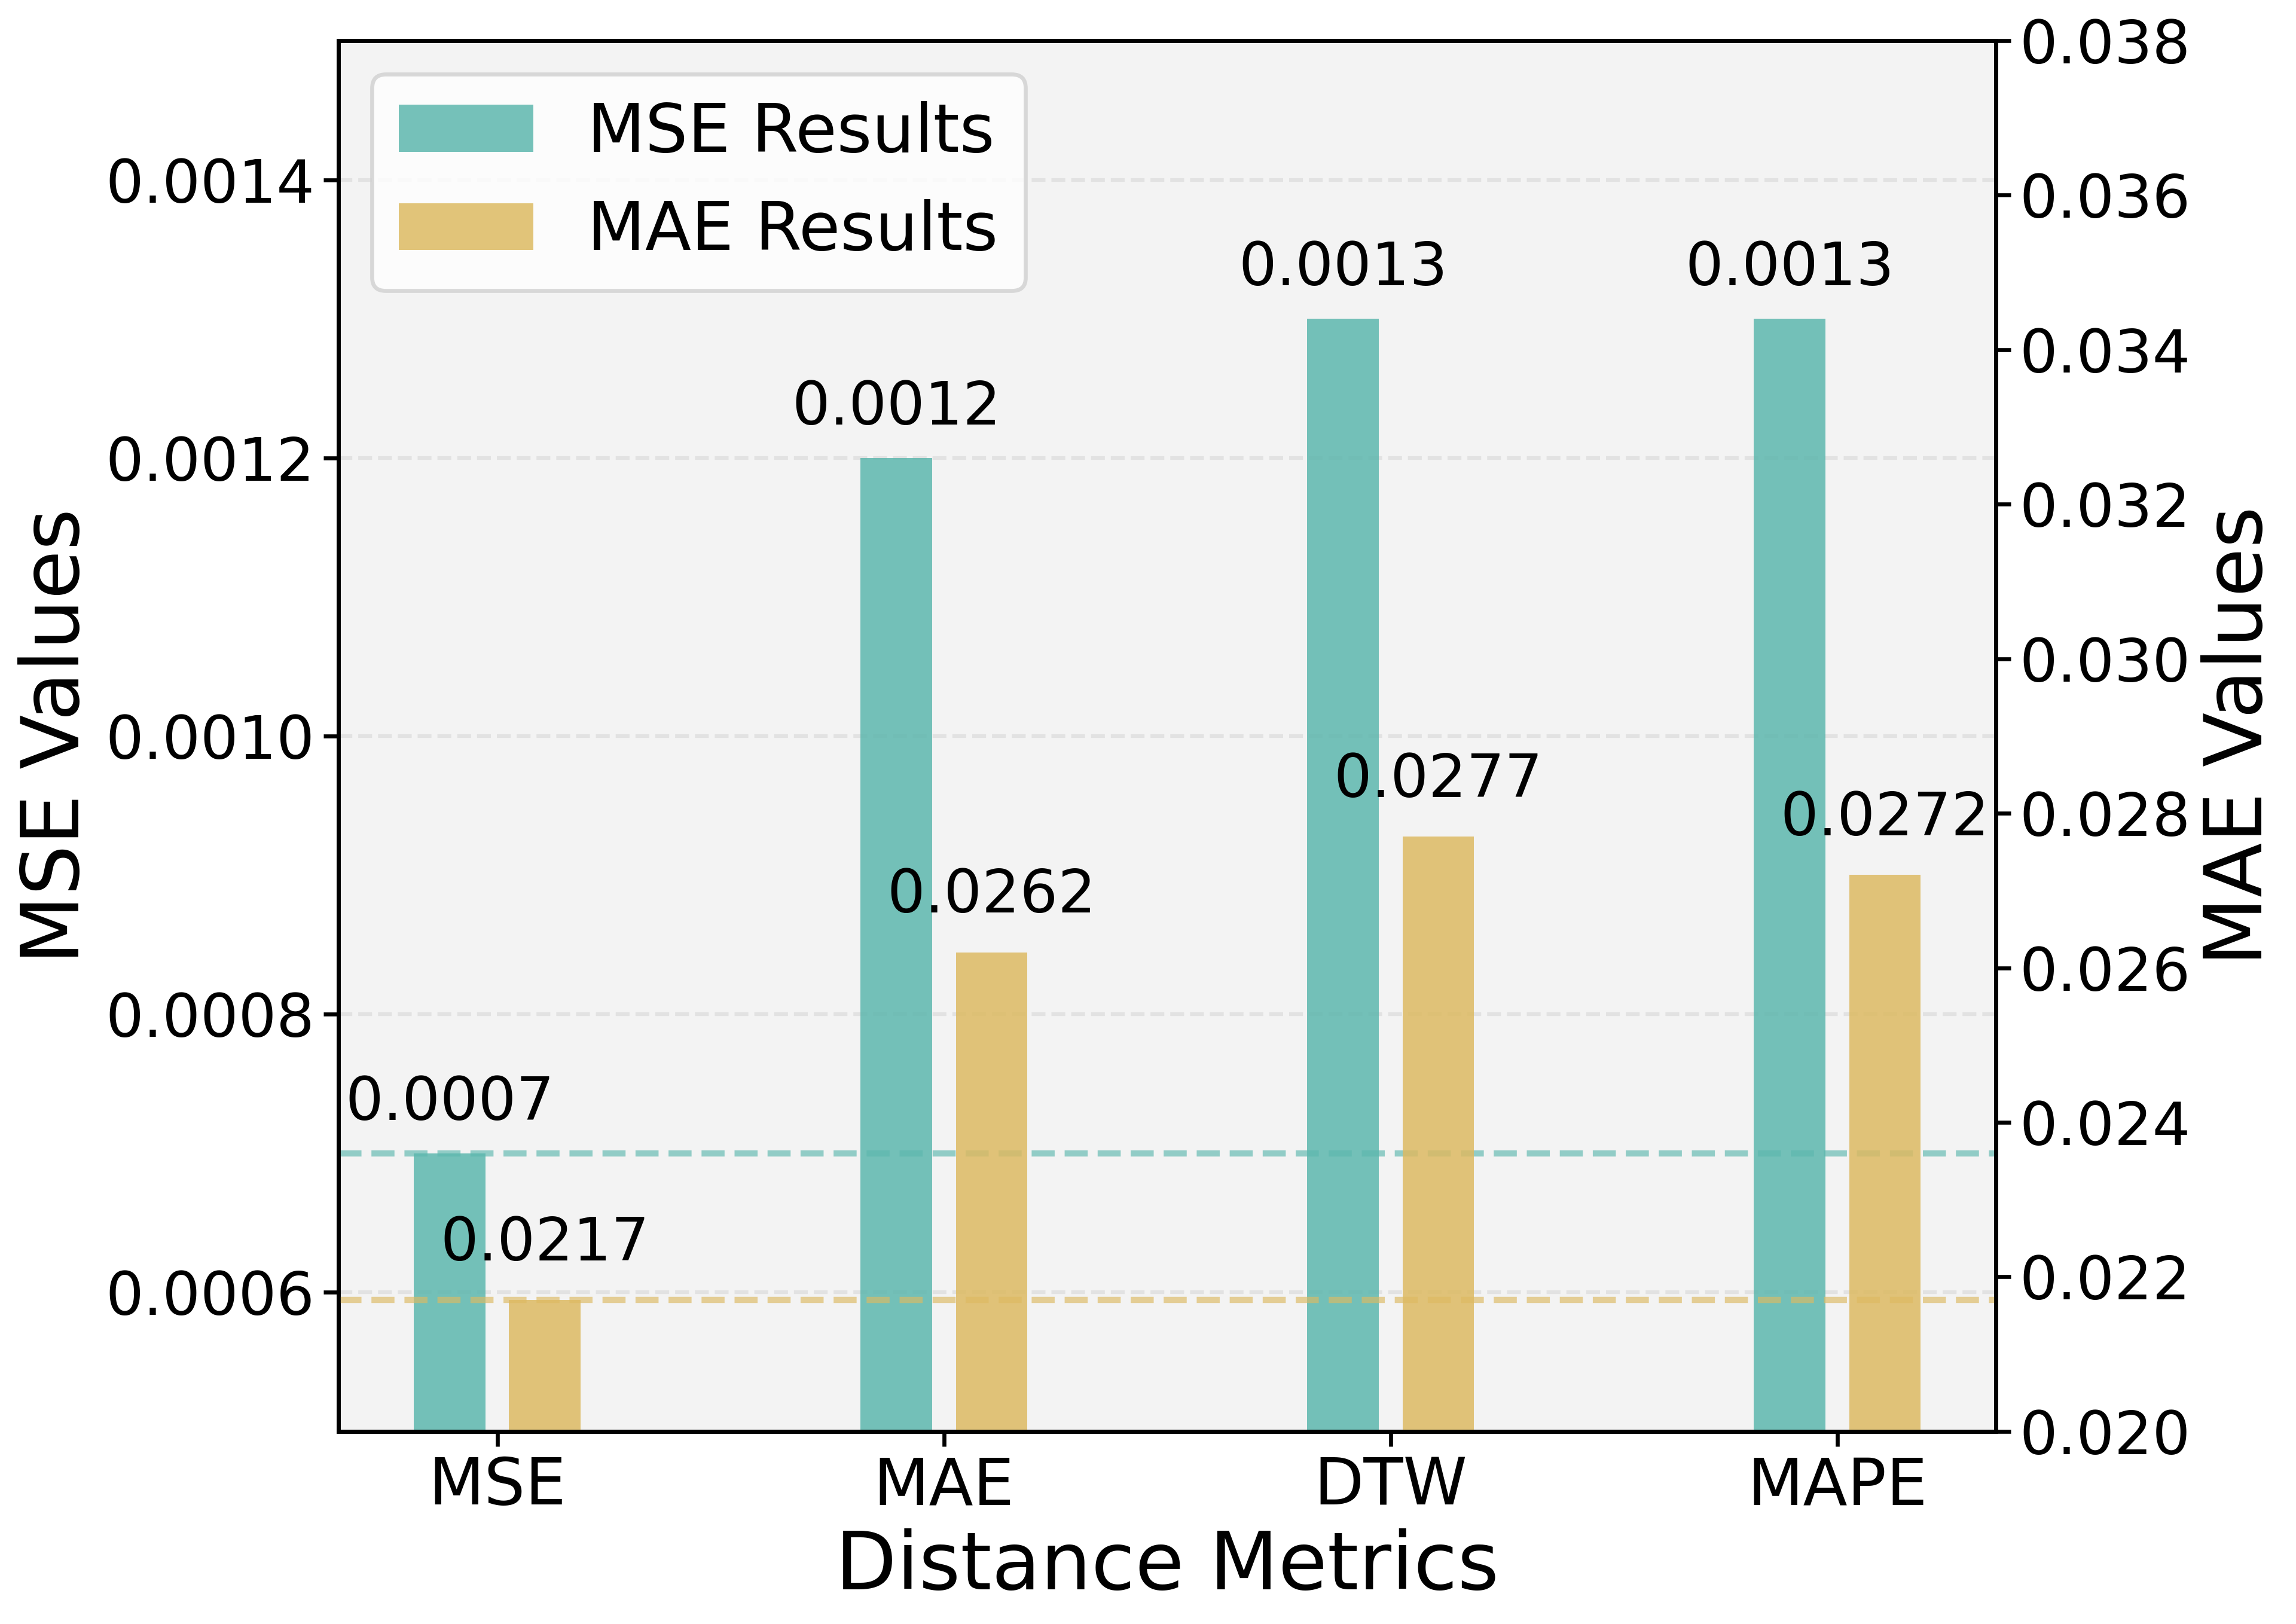
\includegraphics[width=0.32\textwidth]{images/distance/NASDAQ_results.png}
    \vspace{-0.1in}
    \caption{Experimental results based on MSE, MAE, DTW, MAPE Distance Metrics.} 
    \label{fig:distance_metrics}
    \vspace{-0.1in}
\end{figure*}


% \input{images/6_ts_case}
% \begin{figure}[ht]
%     \centering
%     \includegraphics[width=1.0\linewidth]{images/appendix_2_zyt.pdf}
%     \caption{Completion number \textit{vs.} (left) MSE $\downarrow$ and (right) MAE $\downarrow$. Experiments are conducted on ETTh1 using Qwen2.5B-7B-Instruct.}
%     \label{fig:mse}
% \end{figure}

% \subsection{Visualization of Prediction Results}
% In this visualization (Figure \ref{fig:ts_case}), \Ours is compared against six baseline methods, including LLM-based approaches (GPT4TS and TimeLLM) and traditional models (PatchTST, iTransformer, Autoformer, and TimeXer). \Ours consistently demonstrates more accurate and smoother predictions, closely aligning with the ground truth. In contrast, the version of \Ours trained with only SFT performs poorly, yielding subpar forecasting results. On the other hand, \Ours with only RL achieves improved performance, outperforming the baselines to some extent.



% \subsection{Impact of Predicted Window Length}
% \input{table/4_predicted_window_length}

% The results in Table \ref{tab:predicted_window} demonstrate that \Ours consistently outperforms TimeLLM across multiple datasets and prediction horizons, particularly in long-sequence rolling forecasting tasks. Our approach employs a rolling prediction strategy: first using the historical 96 time steps to predict the subsequent 96 steps, and then recursively feeding the predicted values back as input to forecast further into the future. In the ETTh1 dataset, \Ours achieves an MSE of 6.4146 and an MAE of 1.2693 under the 192-step forecasting window, substantially lower than TimeLLM’s MSE of 7.7990 and MAE of 1.4989, highlighting its superior capability in multi-step rolling prediction. Under the longer 336-step forecasting window, \Ours obtains an MSE of 6.6886, still significantly outperforming TimeLLM’s MSE of 9.3575, which indicates that the model maintains high accuracy and stability even after multiple recursive prediction steps.
% Overall, although TimeLLM shows certain competitiveness in short-term forecasting tasks, \Ours demonstrates stronger generalization performance and practicality as the prediction horizon increases, thanks to its more effective temporal modeling and rolling forecasting mechanism.

% \input{table/9_memory_time}
% \subsection{Trade-off Between Accuracy and Inference Efficiency}


% While the gains in Table \ref{tab:main_results_mse} appear modest, they stem from a paradigm prioritizing reasoning depth, interpretability, and generalization over speed. As shown in Table~\ref{tab:efficiency}, Time-R1 (2.93 samples/s, 22,502 MB) incurs high cost due to its LLM-based multi-step reasoning, unlike the lightweight PatchTST (790.30 samples/s, 583 MB). This "slow-thinking" design is intentional, targeting high-impact, latency-tolerant applications—such as financial, energy, or environmental forecasting—where accuracy and trust matter more than real-time response. Time-R1 offers interpretable reasoning, strong generalization, and a foundation for future improvements, making it suitable for scenarios where decisions are costly and explanations are essential.



% \subsection{Visualization of Prediction Results}
% In this visualization (Figure \ref{fig:ts_case}), \Ours is compared against six baseline methods, including LLM-based approaches (GPT4TS and TimeLLM) and traditional models (PatchTST, iTransformer, Autoformer, and TimeXer). \Ours consistently demonstrates more accurate and smoother predictions, closely aligning with the ground truth. In contrast, the version of \Ours trained with only SFT performs poorly, yielding subpar forecasting results. On the other hand, \Ours with only RL achieves improved performance, outperforming the baselines to some extent.
% \input{images/6_ts_case}

% \subsection{Case Study: an Input and Output Example of \Ours}
% % We provide a complete input-output example of \Ours for reference, with some time steps omitted, shown in Table \ref{tab:full_data}.


% Table~\ref{tab:full_data} presents a concrete instance of Time-R1 performing inference on the ETTh1 dataset. Unlike traditional "fast-thinking" models that directly map historical data to future values, Time-R1 initiates a deliberate reasoning phase enclosed within <think> tags. As illustrated, the model effectively decomposes the time series logic: it first identifies key statistical properties, observing a clear upward trend where daily peaks rise from 7.4 to 12.7, and characterizes the daily seasonality with specific descriptions of night troughs and morning peaks.

% Furthermore, the generated thought process demonstrates a structured forecasting strategy. The model explicitly articulates its method—using the final observed day as a baseline with incremental adjustments—while critically evaluating the uncertainty caused by the limited history window. This interpretable intermediate step ensures that the final numerical predictions in the \texttt{<answer>} block are not merely statistical extrapolations, but the result of a logical derivation that aligns domain knowledge with observed temporal dynamics.

% \input{table/7_full_data}

% \section{Limitations}
% \label{limitation}
% Despite significant advancements in enhancing the model’s ability to capture high-frequency temporal patterns and improve time series reasoning, challenges remain due to computational limitations that prevent experimentation with larger open-source models. Additionally, extending the length of the prediction window is not feasible. Consequently, our method may encounter inaccurate predictions when dealing with complex temporal structures or long-term forecasting requirements.




% \section{Broader Impact}
% \label{broader_impact}
% This paper presents work whose goal is to advance the field of Machine Learning. There are many potential societal consequences  of our work, none which we feel must be specifically highlighted.

